\chapter{Dynammic Programming}
    \section{Fast Knapsack 3k trick}
        Suponha que você tem um conjunto $A$ com $N$ valores e $\sum_{i=0}^{N-1} a[i] = M$.
        Queremos calcular quais possiveis somas podemos obter.
        
        Primeiro, se todos os valores são distintos $N < \sqrt(M)$.
        
        Se não são, podemos representar os $K$ caras iguais a $x$ como sendo $x, 2*x, 4*x$ até o maior $2^i < K$ assim esses elementos representaram a mesma soma que os anteriores.
        Chegando numa solução que tem complexidade $O(M*\sqrt(M)$. se for só um subset sum, podemos ainda usar um bitset.
        
        Exemplo 1:
        
        You are in a book shop which sells $n$ different books. You know the price $h[i]$, the number of pages $s[i]$ and the number of copies of each book $k[i]$.

        You have decided that the total price of your purchases will be at most $x$. What is the maximum number of pages you can buy? You can buy several copies of the same book.
        \lstinputlisting{./solutions/DP/BookShopII.cpp}
        
        Exemplo 2:

        A group of $n$ children are coming to Helsinki. There are two possible attractions: a child can visit either  (zoo) or  (amusement park).

        There are m pairs of children who want to visit the same attraction. Your task is to find all possible alternatives for the number of children that will visit zoo. The children's wishes have to be taken into account.
        \lstinputlisting{./solutions/DP/SchoolExcursion.cpp}
    \section{SOS DP}
        Sum over subsets (SOS) DP is a trick that allows you to efficiently compute the sum of all the subsets of an array.

        The naive solution would be to iterate through every pair of masks and check if one of them is a subset of the other.
        We can speed this up if we iterate over only subsets of the current mask and add up all of the those values to get the sum over subsets for a particular mask.

    The difference comes from the fact that in the first example we iterate over every pair of subsets which takes $(2^n)^2$ time and the second we iterate directly over the subsets for each mask. This means each mask is only visited by $2^{n - k}$ other masks where k is the number of elements of the mask.
    
    This means that the total time complexity is O($\sum_{0}^{n} {n \choose k} \cdot 2^{n - k} = 3^n$).

    Notice how in both of these examples we don't seem to be saving much information between different subsets which is the essence of DP.
    Define $\texttt{SOS}(\texttt{mask}, x)$ to be the sum of subsets of mask such that the first $x$ bits of the subset are identical to the first $x$ bits of mask.
    For example, $\texttt{SOS}(1001001, 3)$ includes the subsets $1001001$, $1000001$, $1001000$, $1000000$ which all have the same common prefix of $100$.
    

    $\texttt{SOS}(mask, x) = \left\{  \begin{array}{ c l }  \texttt{SOS}(\texttt{mask}, x - 1) + \texttt{SOS}(\texttt{mask} - 2^i, x - 1) & \quad \textrm{if } |2^i \wedge \texttt{mask}| > 0 \\  \texttt{SOS}(\texttt{mask}, x - 1) & \quad \textrm{otherwise}  \end{array} \right.$

    Example:
    Given a list of $n$ integers, your task is to calculate for each element x:
    
    \begin{itemize}
        \item the number of elements $y$ such that $x|y=x$, can be seen as $y \subseteq x$.
        \item the number of elements $y$ such that $x\&y=x$, that is equal to $!x|!y=!x$, can be seen as $!y \subseteq !x$.
        \item the number of elements $y$ such that $x\&y\neq0$, that is the complement of to $!x|y=!x$, can be seen as $y \subseteq !x$.
    \end{itemize}

    solution of the problem is $O(X)$, where $X$ is the greates element in $n$.
    
    \lstinputlisting{./solutions/DP/BitProblem.cpp}
    
    \section{Permutation Trick}

    suppose u have to count something over permutations. It can be modelled as:

    $DP[i]$ counting over permutations with $i$ elements.
    The main idea is to iterate $j$ over $1$ to $i$, and we say that element $i$ was positioned at $j$, and move every other to the right, dealing with the counting in the process.

    Example: 
    
    Your task is to count the number of permutations of $1,2, \ldots ,n$ that have exactly $k$ inversions.

    $DP[i][j] =$ permutations with $i$ elements and $j$ inversions.
        
    $DP[i][j] =  \sum_{k = 0}^{i} dp[i-1][j-(i-k)]$

    In the problem u need to do some optimizations with prefix sum.

    \lstinputlisting{./solutions/DP/PermutationInversions.cpp}

    \section{Open Interval Trick}

    Suppose u have to count something over multiple intervals, and each element need to be added to some interval.  Suppose they are sorted.

    $DP[i][k]$ counting with the first i elements added and there are k intervals "open".
    the main idea is to iterate $j$ over $1$ to $i$, and we say that element $i$ was positioned at $j$, and move every other to the right, dealing with the counting in the process.

    Example: 
    
    Your company has $n$ coders, and each of them has a skill level between $0$ and $100$. Your task is to divide the coders into teams that work together.

    The penalty for creating a team is the skill level difference between the best and the worst coder.

    In how many ways can you divide the coders into teams such that the sum of the penalties is at most $x$?

    We just need another state to $x$, and then do the combinations.

    \lstinputlisting{./solutions/DP/PermutationInversions.cpp}

    % \section{Slope Trick}
    % TBD - https://usaco.guide/adv/slope-trick?lang=cpp

    \section{Dp Optimizations}

    \begin{table}[h]
    \centering
    \begin{tabular}{|p{1.5cm}|c|p{4.3cm}|p{1.5cm}|p{1.9cm}|}
    \hline
    \textbf{Name} & \textbf{Original Recurrence} & \textbf{Sufficient Condition of Applicability} & \textbf{Original Complexity} & \textbf{Optimized Complexity} \\
    \hline
    \small Convex Hull Optimization1 & $dp[i] = min_{j<i}\{F[j] + b[j] * a[i]\}$ & $b[j] \geq b[j + 1]$ and $a[i] \leq a[i + 1]$ & $\mathcal{O}(n ^ 2)$ & $\mathcal{O}(n)$ or $\mathcal{O}(n log(n))$ w/ line container\\
    \hline
    % \small Convex Hull Optimization2 & Row 2, Col 2 & Row 2, Col 3 & Row 2 & Row 1 \\
    % \hline
    \small Divide and Conquer Optimization & $dp[i][j] = min_{k < j}\{dp[i - 1][k] + C[k][j]\}$ & $A[i][j] \leq A[i][j + 1]$ & $\mathcal{O}(kn^2)$ & $\mathcal{O}(knlog(n))$ \\
    \hline
    \small Knuth Optimization & $dp[i][j] = min_{i < k < j}\{dp[i][k] + dp[k][j]\} + C[i][j]$ & \scriptsize $A[i][j-1] \leq A[i][j] \leq A[i+1][j]$ & $\mathcal{O}(n ^ 3)$ & $\mathcal{O}(n ^ 2) $ \\
    \hline
    \end{tabular}
    \caption{}
    \end{table}

    \begin{itemize}
        \item $A[i][j]$ — the smallest k that gives optimal answer, for example in $dp[i][j]=dp[i-1][k]+C[k][j]$.
        \item $C[i][j]$ — some given cost function.
        \item $F[j]$ - Value computed in constant time, frequently will be equal to $dp[j]$.
    \end{itemize}
    
    % 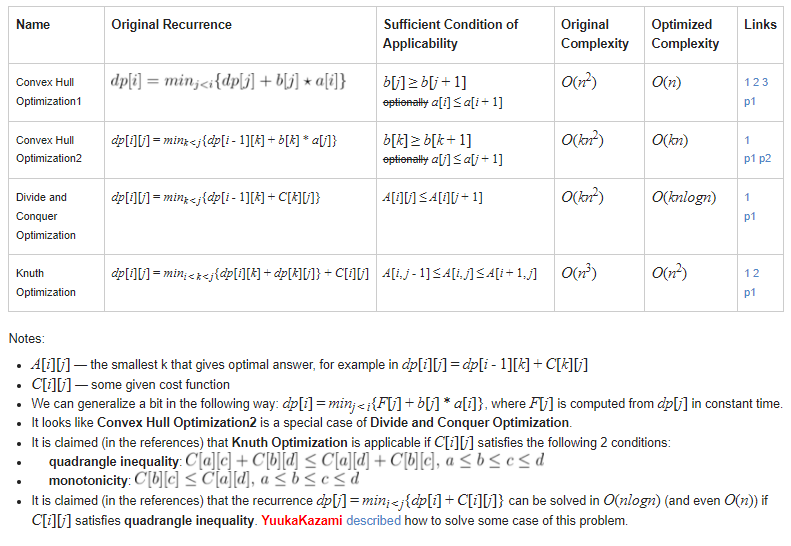
\includegraphics{solutions/DP/dpo.png}
    \subsection{D\&C}
    
    \lstinputlisting{./solutions/DP/divideandconquer.cpp}
    \subsection{Knuth Optimization}
    \lstinputlisting{./solutions/DP/knuth_optimization.cpp}
    \subsection{Convex Hull Trick}
        \subsubsection{Convex Hull Trick 1}
        This solutions only works when the coefficients are all increasing / decreasing, and the queries decreasing / increasing. Improve $O(n^2)$ to $O(n)$. (Original Problem: Codeforces - Round 189 (Div. 1) C)
        \lstinputlisting{./solutions/DP/ConvexHull1.cpp}
        
        \subsubsection{Convex Hull Trick 2}
        This solutions works under the same conditions for Convex Hull Trick 1, but it's used to solve problems in a 2D dynamic programming, like problem NKLEAVES from spoj. In resume we need to group $N$ leaves in $K$ groups, for each coordinate between 1 and $N$ there is a leaf with weight $w_i$, and the leaves can only be moved to the left, and the cost is $w_i * d$ where $d$ is the distance that leaf $i$ was moved. The problem asks for minimum cost to group the $N$ leaves in $K$ groups. Lets reverse the leaves weights, now the leafs can only be moved to the right.
        
        So, the recurrence is:
        
        \bigskip
        
        $dp_{i, j} = \min_{k \leq i} ( (\sum_{p=k}^{i} (i - p) * w_p) + dp_{k - 1, j - 1})$, clearly $O(n^2k)$
        
        \bigskip
        
        So we will keep our lines in such way, that we can solve this problem, see the code below. 
        
        This solutions only works when the coefficients are all increasing / decreasing, and the queries decreasing / increasing. Improve $O(n^2k)$ to $O(nk)$. (Original Problem: SPOJ - NKLEAVES)
        
        \lstinputlisting{./solutions/DP/ConvexHullTrick2.cpp}
        
        \subsubsection{Convex Hull Trick 3 (Online Queries)}
        This solutions works without any assumption about the coeficients, in this case we will query is answered in $O(logn)$.
        
        Improve $O(n^2)$ to $O(nlogn)$. (Original Problem: Codeforces - Round 463 div1+div2 F. Escape Through Leaf)
        
        \lstinputlisting{./solutions/DP/ConvexHullTrick3.cpp}
        
    \section{Steiner Tree DP}

    MST for a subset
    
    \lstinputlisting{./solutions/DP/SteinerTree.cpp}
    